\chapter{Boundary conditions, numerically}
\label{ch:c2}
\begin{keybox}
\textbf{Key idea.} A boundary condition is not an afterthought bolted
onto a solved interior --- it is baked into the weak form, and the
\emph{way} it is imposed decides what the simulation conserves. A
no-flux (natural) boundary costs nothing to impose and conserves mass
exactly; a Dirichlet boundary is imposed by replacing rows and
\emph{deliberately} breaks conservation, because it lets material cross
the boundary.
\end{keybox}

This concept shows, with measured numbers, how the two boundary
treatments the Cahn--Hilliard brick supports are imposed and what each
one costs and means. It connects to Physics Chapter~\ref{ch:p1} (whose
spinodal runs are all no-flux) and to the manufactured-solution study of
Chapter~\ref{ch:c1} (which needed Dirichlet data).

\section{Boundaries live in the weak form}

Multiply the conserved dynamics \eqref{eq:ch} by a test function $w$ and
integrate by parts:
%
\begin{equation}
  \intv w\,c_t\;+\;M\!\intv \grad w\cdot\grad\mu
  \;=\; M\!\oint_{\partial\Omega} w\,(\grad\mu\cdot\mathbf n)\,dS .
  \label{eq:weakbc}
\end{equation}
%
The entire influence of the boundary is that one surface integral. What
you do with it \emph{is} the boundary condition.

\paragraph{Natural (no-flux).}
Setting $\grad\mu\cdot\mathbf n=0$ makes the surface term vanish, and
you impose it by \emph{doing nothing} --- simply omit the integral. This
is why it is called \emph{natural}: it is the condition the weak form
adopts on its own. Physically it is a zero-flux wall: no mass crosses
$\partial\Omega$, so total mass $\intv c\,dV$ is conserved to solver
tolerance. Every spinodal run in Physics Chapter~\ref{ch:p1} is a
no-flux run, which is why its mass drift was machine epsilon.

\paragraph{Dirichlet (fixed value).}
To hold the boundary composition at a prescribed $g$ we cannot use the
surface term --- we \emph{replace} the boundary rows of the assembled
system with the identity, $\;A_{ii}\!\leftarrow\!1$, right-hand side
$\leftarrow g - x_i$ (the Newton-increment form). This pins $(c,\mu)$ at
those nodes exactly. It is the treatment the manufactured-solution study
of Chapter~\ref{ch:c1} needed (the exact field is not no-flux), and it
models a composition held fixed at a contact. Crucially, a pinned
boundary \emph{is} a reservoir: whatever flux is needed to maintain the
value flows freely, so mass is \textbf{not} conserved --- by design.

\begin{keybox}
\textbf{A boundary condition changes what you conserve.} No-flux
conserves mass because it forbids boundary flux. Dirichlet abandons
conservation because it fixes a value and lets flux adjust. Neither is
``more correct'' --- they model different physical situations (a sealed
domain vs.\ a contact held at a set composition). Choosing wrong gives a
plausible-looking but physically wrong answer.
\end{keybox}

\paragraph{A third kind: wall free energy.}
A real thin film often \emph{wets} its substrate: one component prefers
the wall. That is a surface free energy $\oint g_s(c)\,dS$ added to
\eqref{eq:F}, which makes the natural flux \emph{nonzero} (a Robin-type
wetting condition) rather than pinning a value. It is genuine physics,
but it lives in the multiphase film brick, not this binary
Cahn--Hilliard brick (see \file{docs/dev/2026-07-13-m5-device-assembly.md},
the A2 wall term); we name it here for completeness and use it in the
device track. This tutorial measures the two treatments the binary brick
implements.

\section{Run it}

\begin{runbox}
\textbf{Run it.}
\begin{lstlisting}
cd computational/02_boundary_conditions
python run.py            # both boundary treatments, compared
\end{lstlisting}
It marches the \emph{identical} spinodal blend (same fixed seed) twice
--- once no-flux, once with every box edge pinned to $c=\CtwoWall$ ---
and prints the mass drift and boundary layer of each. Compare with
\file{EXPECTED.md} and Fig.~\ref{fig:c2fields}--\ref{fig:c2mass}.
\end{runbox}

\begin{figure}[h]\centering
  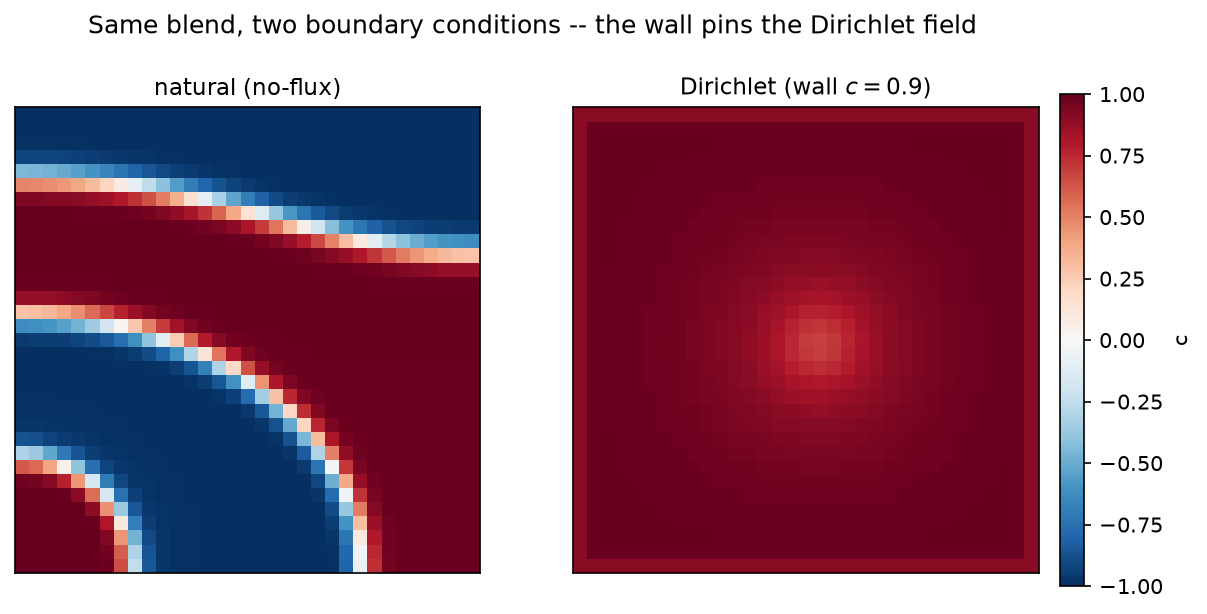
\includegraphics[width=0.92\linewidth]{figures/c2_fields.png}
  \caption{The same blend under the two boundary conditions. Left:
    no-flux --- domains meet the wall freely. Right: Dirichlet ---
    the edge is pinned to $c=\CtwoWall$ and that phase is drawn to the
    boundary, reorganizing the morphology. The measured field
    difference is $\CtwoFieldDiff$ (the full order-parameter range).}
  \label{fig:c2fields}
\end{figure}

\begin{figure}[h]\centering
  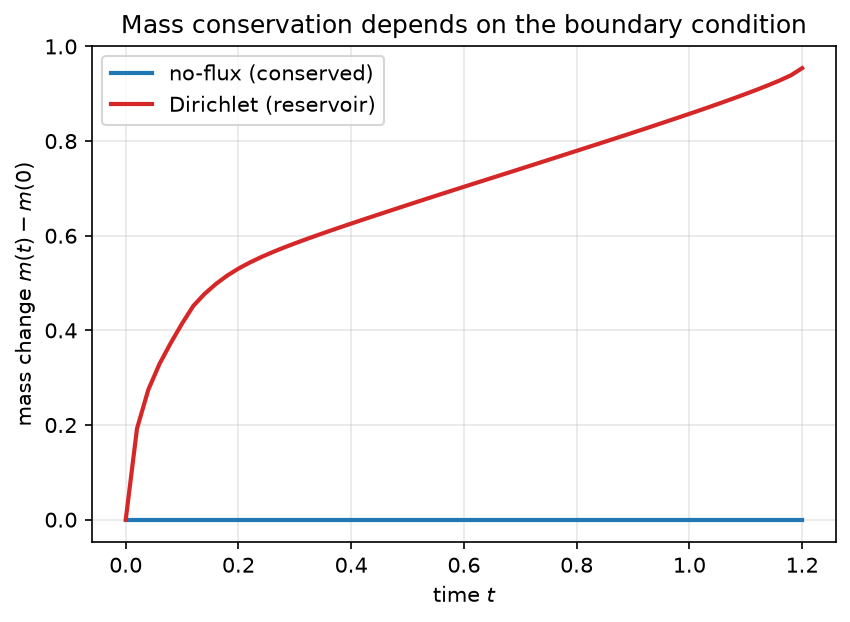
\includegraphics[width=0.7\linewidth]{figures/c2_mass.png}
  \caption{Mass change $m(t)-m(0)$. The no-flux wall conserves mass to
    machine precision (flat at zero); the Dirichlet wall acts as a
    reservoir and draws material in ($\Delta m\approx\CtwoDirMassDrift$).}
  \label{fig:c2mass}
\end{figure}

\begin{keybox}
\textbf{Measured self-check} (fixed seed in \file{bc.py}; field values
are seed-dependent, the conservation/pinning contrast is not).
\begin{center}\small
\begin{tabular}{lcc}
\toprule
 & natural (no-flux) & Dirichlet ($c=\CtwoWall$) \\
\midrule
mass drift $|\Delta m|$ & \CtwoNfMassDrift & \CtwoDirMassDrift \\
edge composition        & \CtwoNfEdge\ (free) & \CtwoDirEdge\ (pinned) \\
field difference max$|c_{\text{nf}}-c_{\text{dir}}|$ & \multicolumn{2}{c}{\CtwoFieldDiff} \\
\bottomrule
\end{tabular}
\end{center}
\end{keybox}

\section{Code walk-through}

The comparison lives in \file{bc.py}, driving the same production brick.

\paragraph{Selecting the boundary.}
\begin{lstlisting}
# natural: pass nothing -- the default weak form is no-flux
st = CahnHilliardStepper(dm, M, kap, dt, order=1)

# Dirichlet: pass the boundary node indices + the data functions
st = CahnHilliardStepper(dm, M, kap, dt, order=1, dirichlet=bidx,
                         gc_fn=lambda x,t: wall, gm_fn=lambda x,t: 0)
\end{lstlisting}
\code{boundary\_free\_nodes} finds the box-edge nodes; \code{gc\_fn},
\code{gm\_fn} supply the pinned $(c,\mu)$ values. The natural case needs
no argument at all --- the load-bearing point of the concept.

\paragraph{Measuring the effect.}
\begin{lstlisting}
m0 = mass(st, st.hist[0])
for _ in range(steps): c, _ = st.step()
drift = abs(mass(st, c) - m0)          # ~1e-16 no-flux; ~0.95 Dirichlet
\end{lstlisting}
\code{mass} integrates $\intv c\,dV$ with the solver's own quadrature ---
the same conservation diagnostic as Physics P1. Running both modes from
the identical seeded initial field isolates the boundary's effect in the
field difference.

\section{Explore on your own}

\question{Sweep the Dirichlet wall value $g\in\{-0.9,0,+0.9\}$. Predict
the sign and rough size of $\Delta m$ for each before running, then
check. For which $g$ is mass \emph{approximately} conserved, and is that
a coincidence of the initial mean?}

\question{Pin only \emph{two} opposite edges (left/right) instead of all
four, leaving top/bottom no-flux. How does the boundary layer and the
mass drift change? This mixed condition is common in device geometries
(contacts on two sides, sealed on the others).}

\question{The no-flux mass drift is $\sim10^{-16}$ --- machine epsilon,
not solver tolerance. Refine the mesh one level and re-measure: does the
drift grow with the number of nodes (accumulated round-off) or stay at
machine level? What does that tell you about how conservation is
enforced here?}

\question{Under Dirichlet, the boundary $\mu$ is pinned to $0$. Is that
physical? Argue what $\mu$ at a composition-pinned contact \emph{should}
be, and why pinning both $c$ and $\mu$ (as this brick does) is a
modelling choice, not a law. What would a $c$-only Dirichlet require of
the solver?}

\question{Estimate the ``cost'' of each boundary condition: count how
many rows the Dirichlet case replaces versus the interior, and argue why
the natural condition is not only physically distinct but computationally
free.}
